\documentclass[Main]{subfiles}
\begin{document}


\chapter{System architectural design}
\section{System functional design}
This section describes the functional design and architecture of the system.
This is also illustrated in Figure \ref{fig:FFD} below.

\begin{figure}[H]
\centering
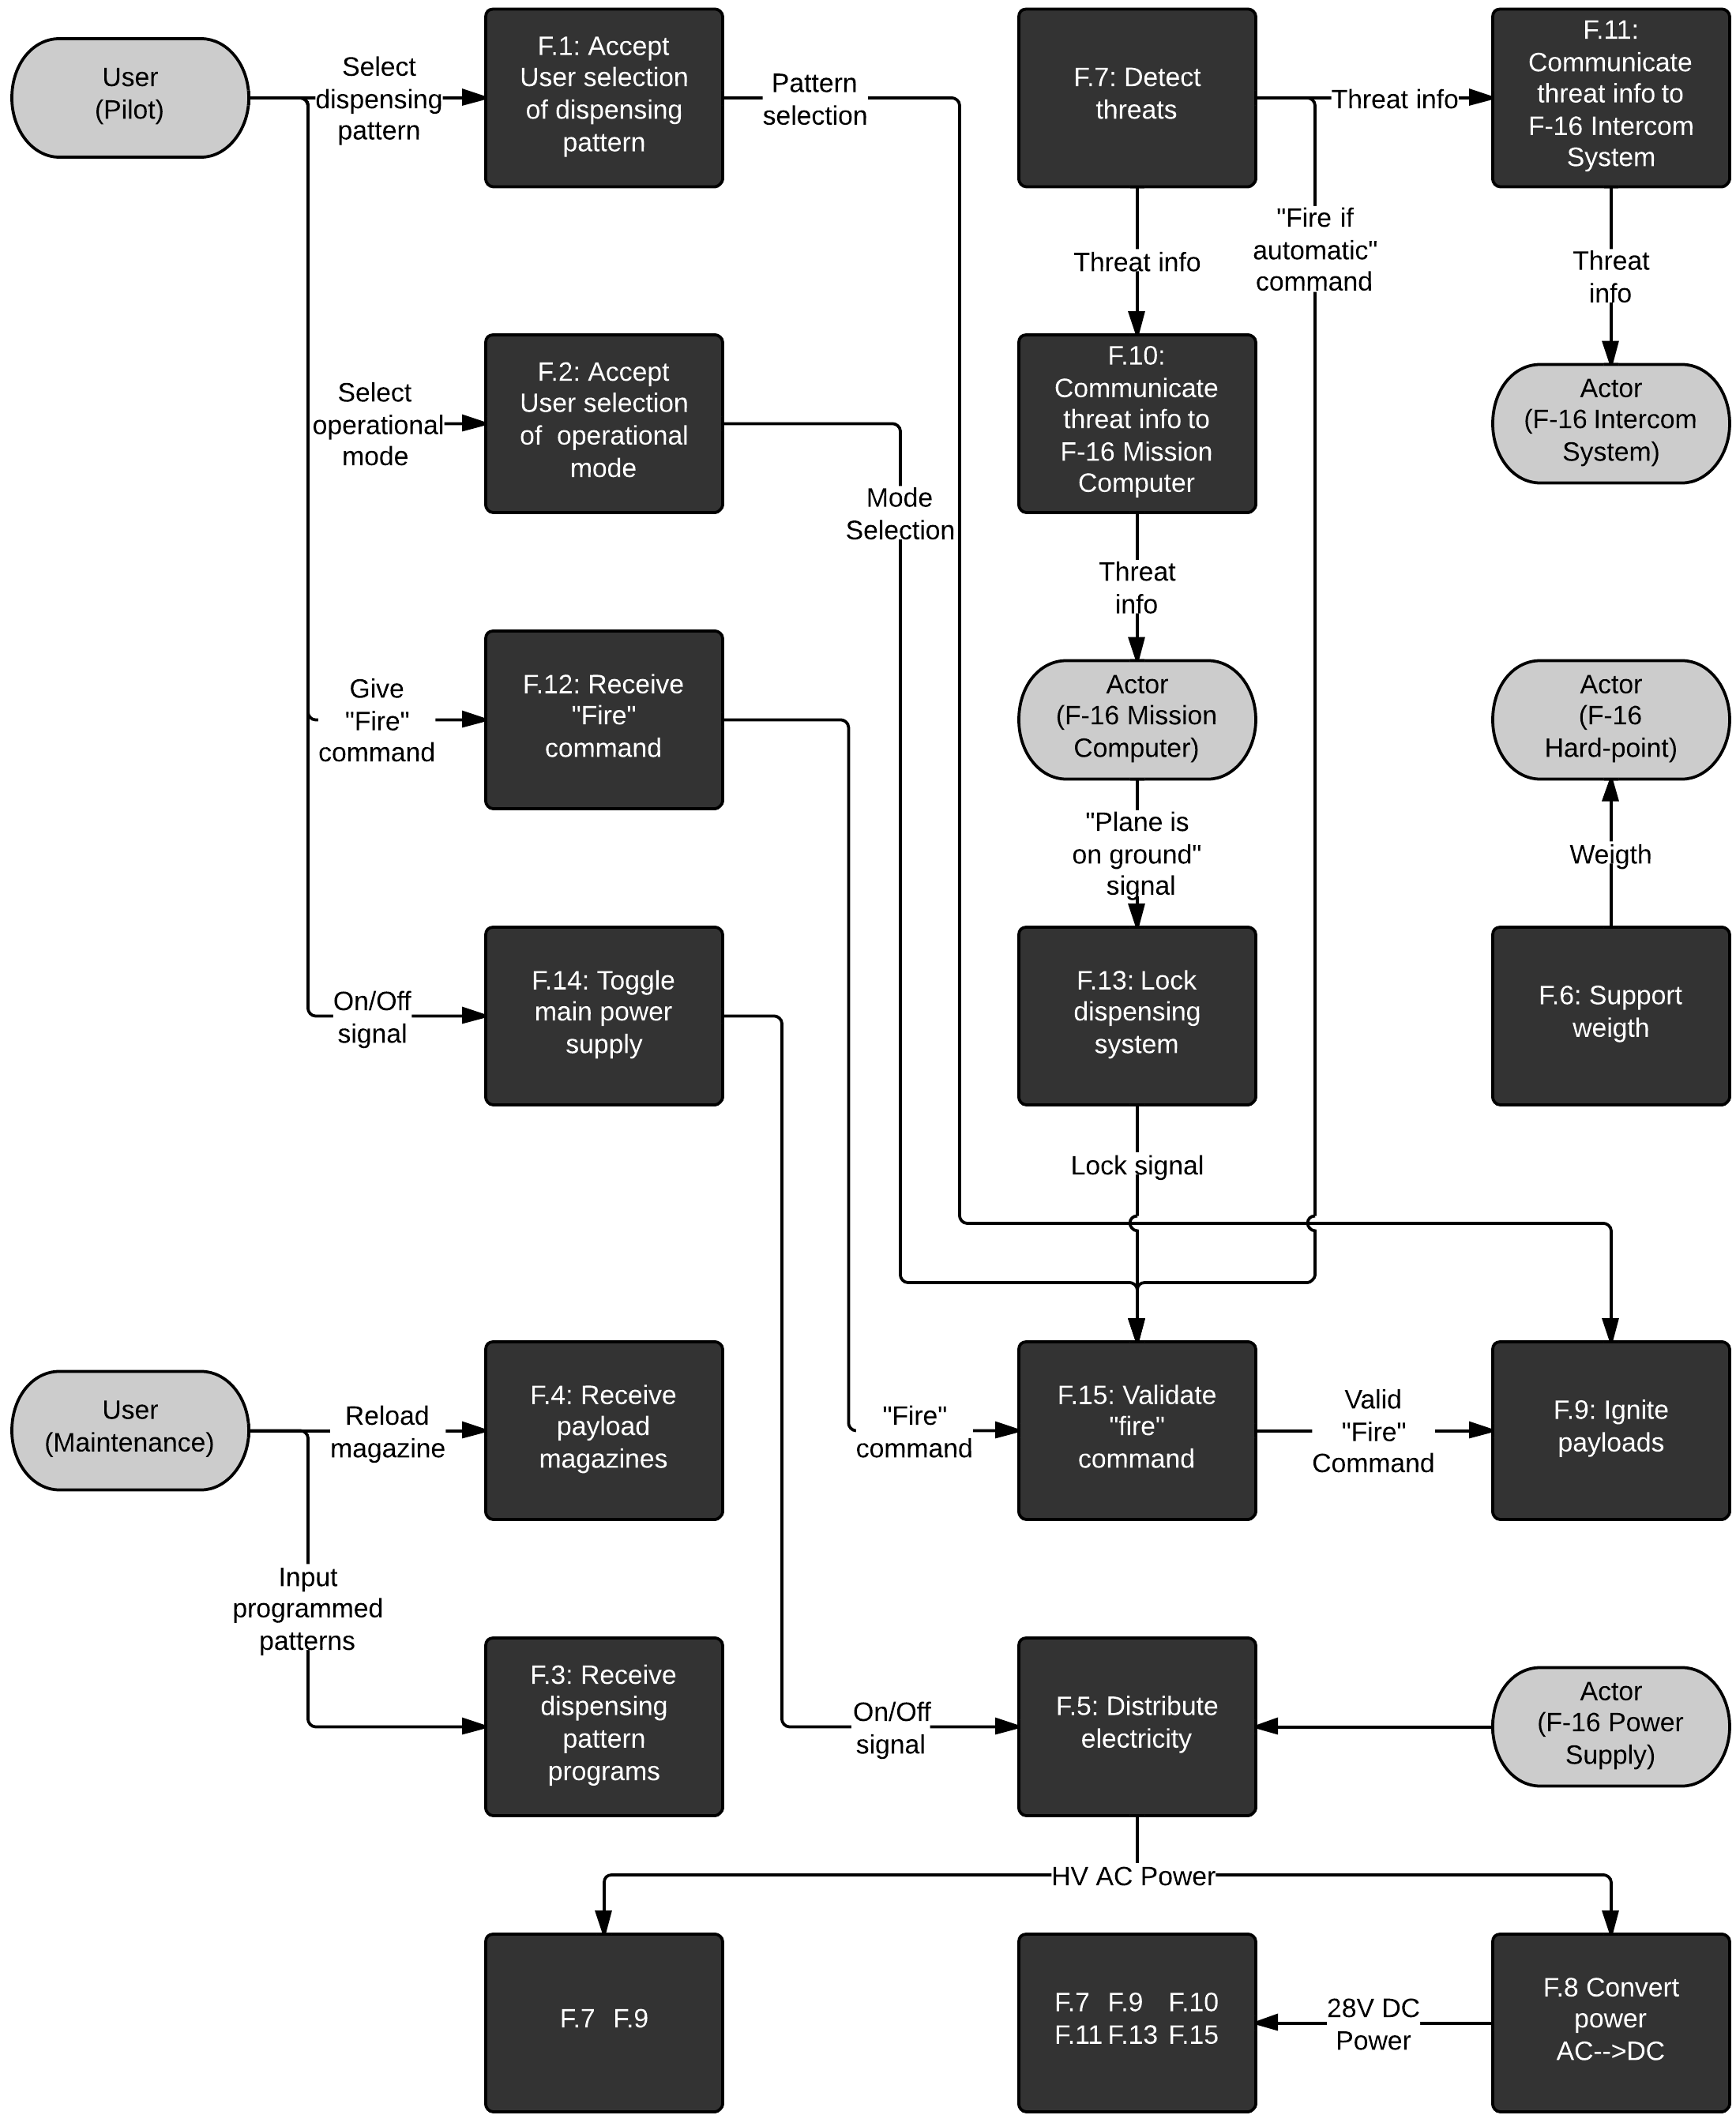
\includegraphics[width=0.80\textwidth]{FunctionalFlowDiagram}
\caption{Functional Flow Diagram}
\label{fig:FFD}
\end{figure}

\subsection{System functions}
\begin{enumerate}[label=F.\arabic*:]
\item Accept User selection of dispensing pattern
\item Accept User selection of operational mode
\item Receive dispensing pattern programs
\item Receive payload magazines
\item Distribute electricity
\item Support weight
\item Detect threats
\item Convert power AC/DC
\item Ignite payloads
\item Communicate threat info to F-16 Mission Computer
\item Communicate threat info to F-16 Intercom System
\item Receive "Fire" command
\item Lock dispensing system
\item Toggle pod power supply
\item Validate "fire" command




\end{enumerate}


In Figure \ref{fig:ComponentsAndInterfaces} an overview of the the complete systems components and interfaces is shown. Each component and interface will described and linked with system requirements in the folllowing sections.

\begin{figure}[H]
\centering
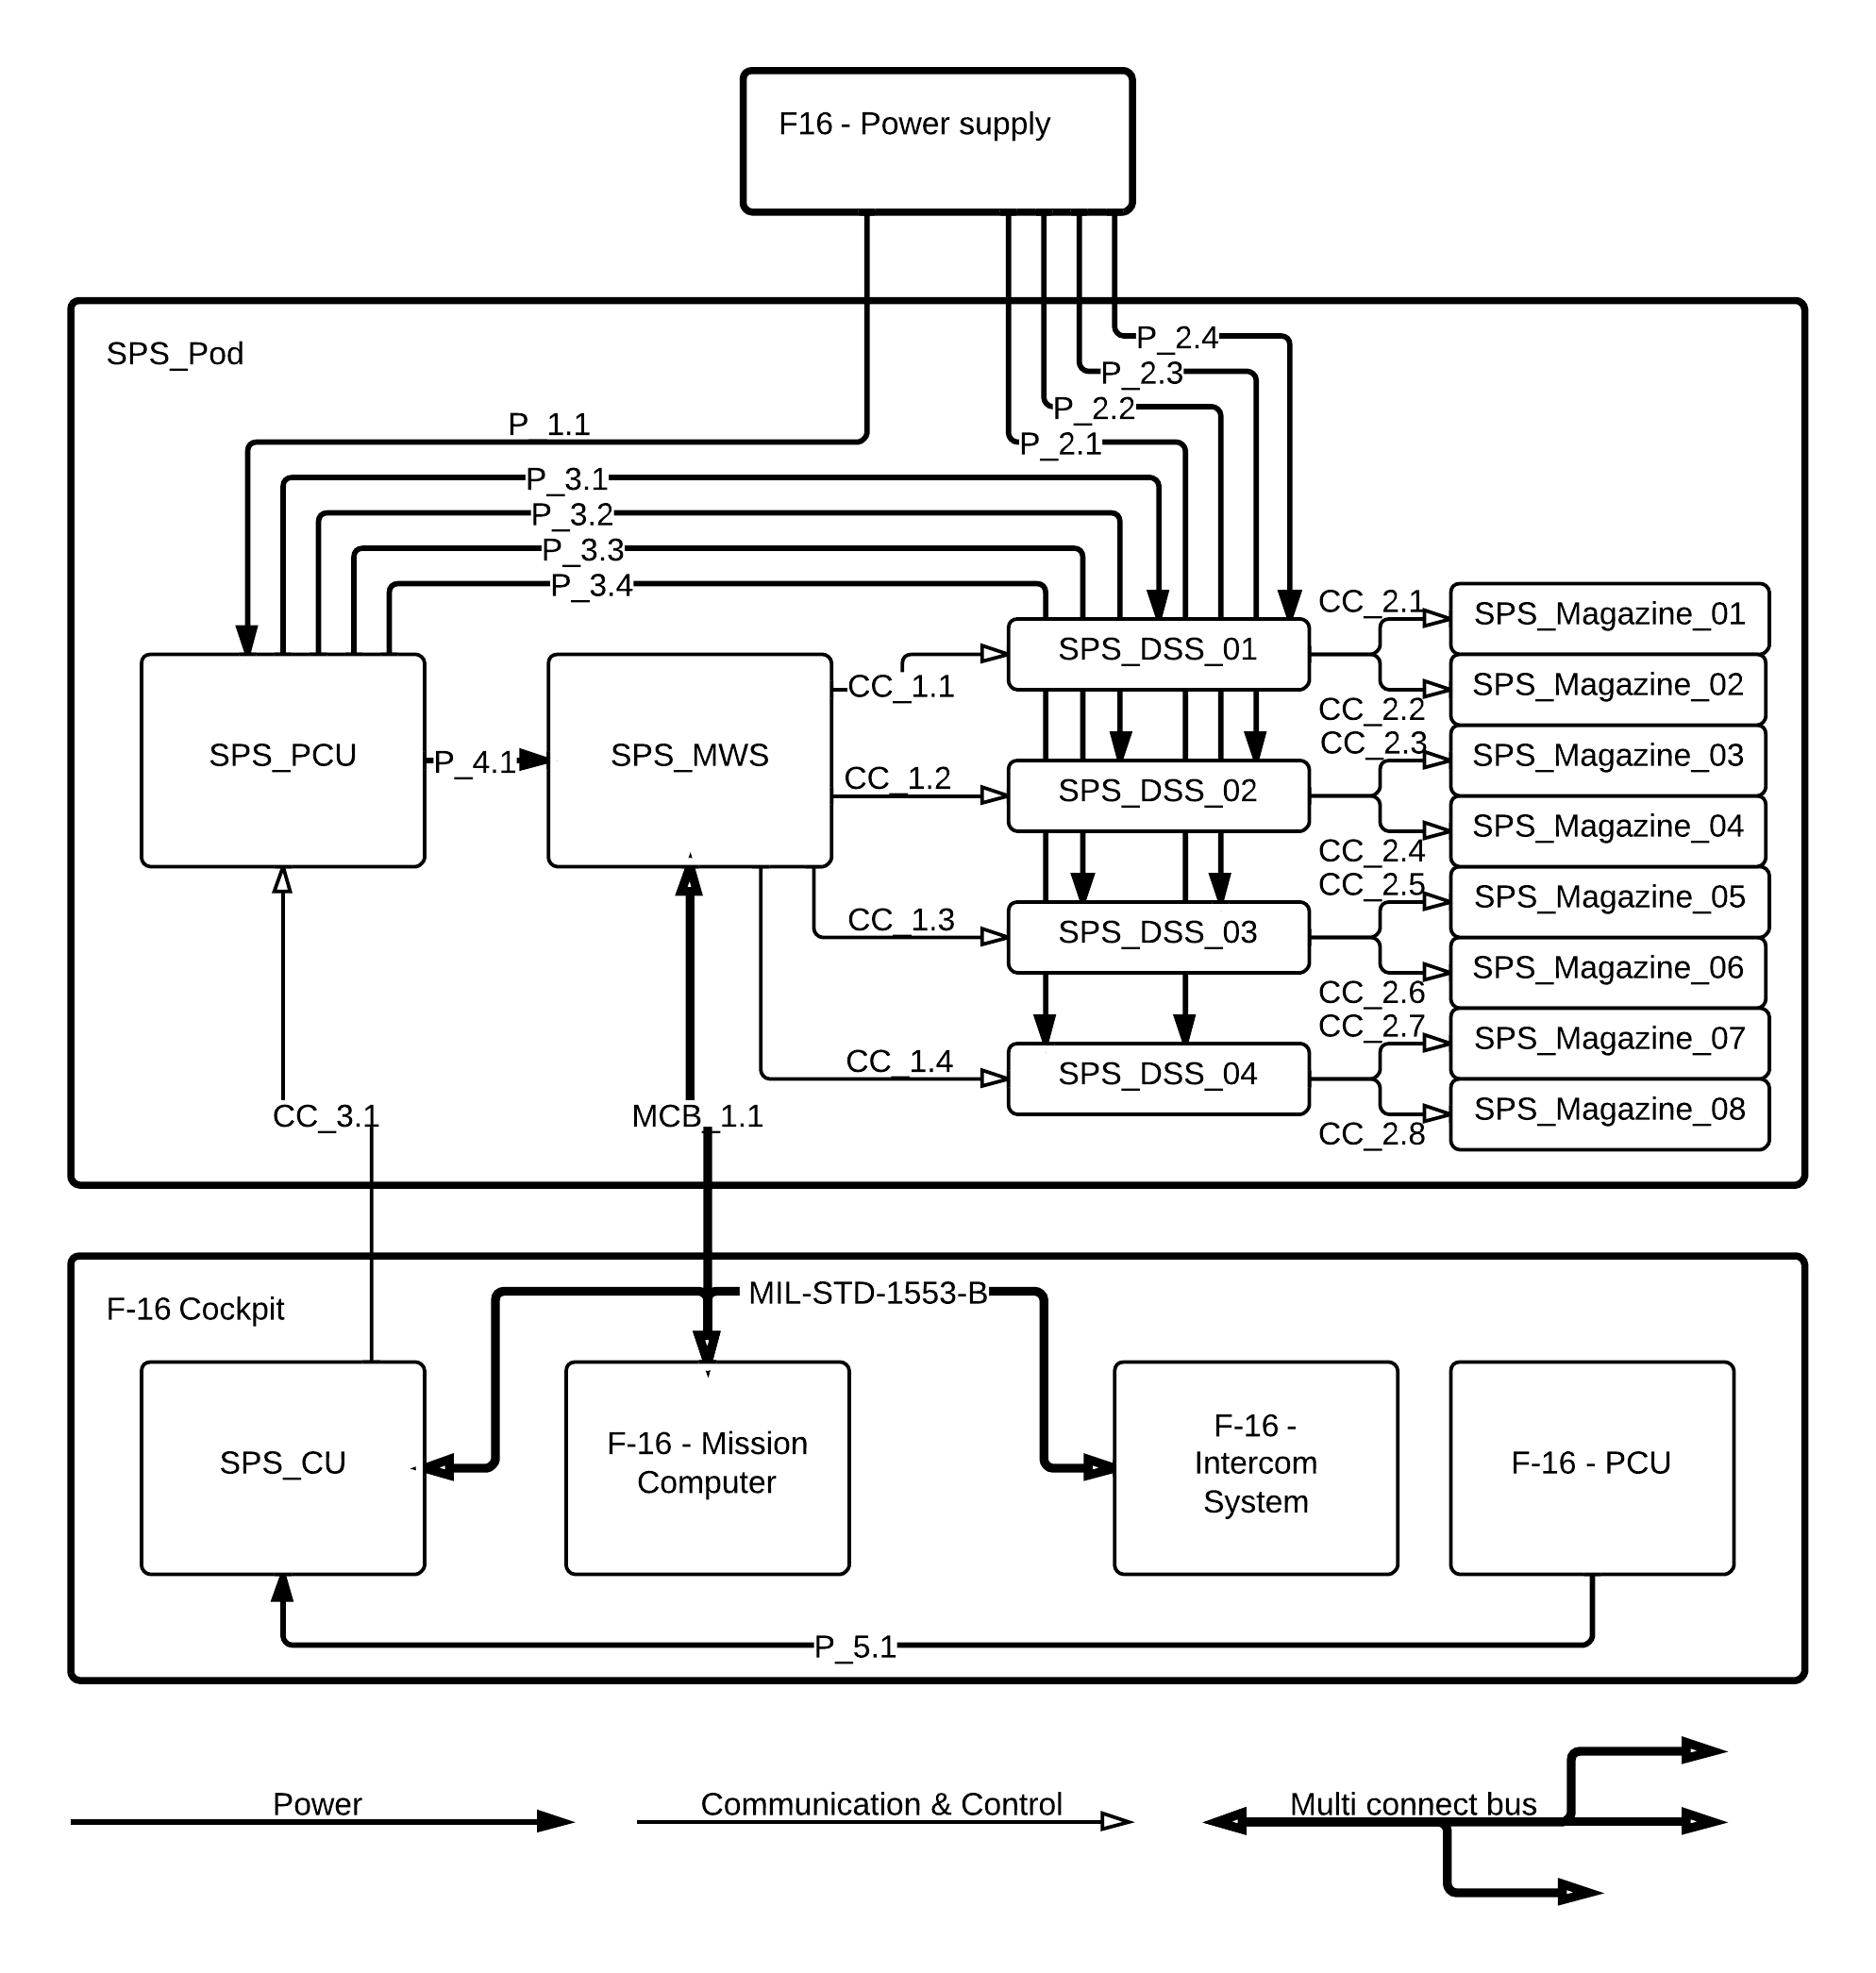
\includegraphics[width = 0.9\textwidth]{ComponentsAndInterfaces}
\caption{Components and interfaces}
\label{fig:ComponentsAndInterfaces}
\end{figure}

\subfile{SystemComponents}
\newpage
\subfile{ConceptOfExecution}
\newpage
\subfile{InterfaceDesign}
\end{document}